%&<tex>
\documentclass[notheorems]{beamer}
\usetheme{Rochester}
%\usefonttheme{serif}

%\usepackage[hmargin=2.5cm, vmargin=2cm]{geometry}
\usepackage{amssymb, mathtools, yhmath, graphicx}
%\usepackage{fontspec, type1cm, titlesec, titling, fancyhdr, tabularx}
%\usepackage{color, unicode-math, float, hhline}
\usepackage{color}
\usepackage{float}

%\usepackage{eulervm}

\usepackage{xpatch}
%\usepackage[abbreviations, per-mode=symbol]{siunitx}
\usepackage[CheckSingle, CJKmath]{xeCJK}
\usefonttheme{professionalfonts}
\usepackage{ccfonts}
%\usepackage{CJKulem}
%\usepackage{enumitem}
\usepackage{tikz}
\usepackage{minted}
\setminted{fontsize=\footnotesize, linenos, frame=lines}
%\usemintedstyle{monokai}
%\usepackage{circuitikz}
%\setCJKmainfont[BoldFont=cwTex Q Hei]{cwTex Q Ming}
%\setCJKsansfont[BoldFont=cwTex Q Hei]{cwTex Q Ming}
%\setCJKmonofont[BoldFont=cwTex Q Hei]{cwTex Q Ming}
\setCJKmainfont{Source Han Sans TW}

\def\normalsize{\fontsize{12}{18}\selectfont}
\def\large{\fontsize{14}{21}\selectfont}
\def\Large{\fontsize{16}{24}\selectfont}
\def\LARGE{\fontsize{18}{27}\selectfont}
\def\huge{\fontsize{20}{30}\selectfont}

%\titleformat{\section}{\bf\Large}{\arabic{section}}{24pt}{}
%\titleformat{\subsection}{\large}{\arabic{subsection}.}{12pt}{}
%\titlespacing*{\subsection}{0pt}{0pt}{1.5ex}

%\usepackage{parskip}
%\parindent=24pt
%\parskip=1em

%\DeclarePairedDelimiter{\abs}{\lvert}{\rvert}
%\DeclarePairedDelimiter{\norm}{\lVert}{\rVert}
%\DeclarePairedDelimiter{\inpd}{\langle}{\rangle}
%\DeclarePairedDelimiter{\ceil}{\lceil}{\rceil}
%\DeclarePairedDelimiter{\floor}{\lfloor}{\rfloor}

\newcommand\abs[1]{\left\lvert #1 \right\rvert}

\newcommand{\img}{\mathsf{i}}
\newcommand{\ex}{\mathsf{e}}
\newcommand{\dD}{\mathrm{d}}
\newcommand{\dI}{\,\mathrm{d}}

%\makeatletter
%\def\th@mystyle{%
    %\normalfont % body font
    %\setbeamercolor{block title example}{bg=green,fg=white}
    %\setbeamercolor{block body example}{bg=green!20,fg=black}
    %\def\inserttheoremblockenv{exampleblock}
  %}
%\makeatother
%\theoremstyle{mystyle}
%\newtheorem*{problem}{Problem}

\theoremstyle{definition}
\newtheorem{theorem}{定理}
\newtheorem{lemma}{引理}
\newtheorem{problem}{例題}
\newtheorem{definition}{定義}

\setbeamercovered{transparent}
%\usefonttheme[onlymath]{serif}
%\settowidth{\leftmargini}{\usebeamertemplate{itemize item}}

%\makeatletter
%\patchcmd\beamer@@tmpl@frametitle{\insertframetitle}{\insertsection-\insertframetitle}{}{}
%\makeatother

\title{IOI-camp lecture Math}
\author{Meteor}

\renewcommand*{\emph}[1]{{\bf #1}}

\begin{document}

\begin{frame}
  \titlepage
\end{frame}

\section{Introduction}

\begin{frame}{\secname}
  程式競賽中的數學:

  \begin{itemize}
    \setlength{\itemindent}{2em}
    \item<2-> 數學知識
    \item<3> 數學想法
  \end{itemize}
\end{frame}

\begin{frame}[t]{\secname \ -- 數學知識例子}
  \begin{problem}[平方國的平方幣, TIOJ 1349]
    給你一個正整數 $n$,請找出最小的 $k$,使得存在 $k$ 個平方數 $a_1^2, a_2^2, \cdots, a_k^2$
    使得 $\sum a_i^2 = n$ 。($n \leq 10^7$)
  \end{problem}

  \begin{itemize}
    \item<2-> 一個很極端的「結論題」。
    \item<3-> 所有正整數都可以寫成 $4$ 個平方數的和 (Lagrange 1770)。
    \item<4-> 太結論也不是很有趣……
  \end{itemize}
\end{frame}

\begin{frame}[t]{\secname \ -- 數學知識例子 2}
  \begin{problem}[Taxes, Codeforces 735D]%
    在一個很古怪的國家,如果你賺了 $x$ 元,你就要繳 $d$ 塊錢的稅,其中 $d$ 是 $x$ 的因數且小於
    $n$ 裡最大的一個。

    \medskip
    現在有一個人賺了 $n$ 元,他想把 $n$ 拆成 $n = n_1 + n_2 + \cdots + n_k$ 然後 $n_i$ 各自繳稅,
    請問他最多可以逃過多少稅?($n \leq 2 \times 10^9$)
  \end{problem}

  \begin{itemize}
    \item<2-> Goldbach's conjecture: 大於 $2$ 的偶數都可以寫成兩個質數的和。
  \end{itemize}
\end{frame}

\begin{frame}[t]{\secname \ -- 數學想法例子}
  但大部份還是屬於「數學想法」的問題。

  \pause
  \medskip
  \begin{problem}[2015 ICPC Daejeon regional pE]
    給你一堆數列 $a_1, a_2, \cdots, a_n$,你要找一個排列 $\sigma$,使得
    \[ \max \Big(
      \abs{a_{\sigma(1)} - a_{\sigma(2)}},
      \abs{a_{\sigma(2)} - a_{\sigma(3)}}, \cdots,
      \abs{a_{\sigma(n)} - a_{\sigma(1)}}
      \Big) \]
    最小。 ($n \leq 10^4$)
  \end{problem}

  \pause
  \begin{definition}
    一個大小為 $n$ 的\emph{排列}是一個從 $[1, n]$ 打到自己的一一對應函數。
  \end{definition}
\end{frame}

\begin{frame}[t]{\secname \ -- 數學想法例子}
  解題四部曲:
  \pause

  \begin{enumerate}[<+->]
    \item 嘗試、觀察:在計算紙上多試試
    \item 神猜結論
    \item {\color{gray} (稍微)}證明
    \item 寫 code
  \end{enumerate}
  \pause

  \bigskip
  亂講的,多半要臨機應變,見招拆招。
\end{frame}

\begin{frame}[t]{\secname \ -- 數學想法例子}
  \begin{enumerate}
    \item 嘗試、觀察
    \item 神猜結論
  \end{enumerate}
  \pause

  \begin{figure}
    \centering
    \only<+>{
    \begin{tikzpicture}[scale=0.8]
      \draw[-latex, thick] (0, 0) -- (10, 0);
      \foreach \x [count=\i] in {0.5, 2, 4, 6, 8} {
        \fill (\x, 0) node (\i) {} circle (1.5mm);
      }
      \node at (0, 0) {};
      \draw (1) edge[bend left=50, -latex, thick] (2);
      \draw (2) edge[bend left=50, -latex, thick] (3);
      \draw (3) edge[bend left=50, -latex, thick] (4);
      \draw (4) edge[bend left=50, -latex, thick] (5);
      \draw (5) edge[bend left=50, -latex, thick] (1);
      \node at (5, -3) {應該不是…};
    \end{tikzpicture}
    }

    \only<+>{
    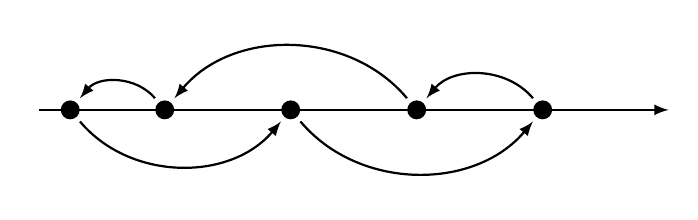
\begin{tikzpicture}[scale=0.8]
      \draw[-latex, thick] (0, 0) -- (10, 0);
      \foreach \x [count=\i] in {0.5, 2, 4, 6, 8} {
        \fill (\x, 0) node (\i) {} circle (1.5mm);
      }
      \node at (0, 0) {};
      \draw (2) edge[bend right=50, -latex, thick] (1);
      \draw (1) edge[bend right=50, -latex, thick] (3);
      \draw (3) edge[bend right=50, -latex, thick] (5);
      \draw (5) edge[bend right=50, -latex, thick] (4);
      \draw (4) edge[bend right=50, -latex, thick] (2);
    \end{tikzpicture}
    }

    \only<+>{
    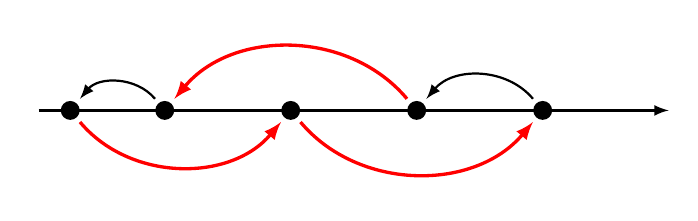
\begin{tikzpicture}[scale=0.8]
      \draw[-latex, thick] (0, 0) -- (10, 0);
      \foreach \x [count=\i] in {0.5, 2, 4, 6, 8} {
        \fill (\x, 0) node (\i) {} circle (1.5mm);
      }
      \node at (0, 0) {};
      \draw (2) edge[bend right=50, -latex, thick] (1);
      \draw (1) edge[bend right=50, -latex, very thick, red] (3);
      \draw (3) edge[bend right=50, -latex, very thick, red] (5);
      \draw (5) edge[bend right=50, -latex, thick] (4);
      \draw (4) edge[bend right=50, -latex, very thick, red] (2);
    \end{tikzpicture}
    }
  \end{figure}
\end{frame}

\begin{frame}[t]{\secname \ -- 數學想法例子}
  \begin{enumerate}
    \setcounter{enumi}{2}
    \item 證明
  \end{enumerate}

  \begin{figure}
    \centering
    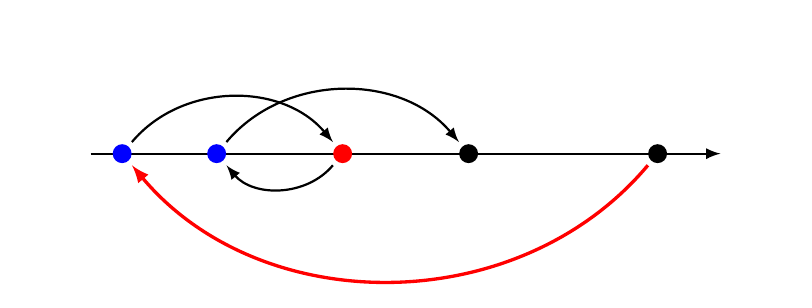
\begin{tikzpicture}[scale=0.8]
      \useasboundingbox (-1, -2) rectangle (11, 2);
      \draw[-latex, thick] (0, 0) -- (10, 0);
      \fill[red] (4, 0) node (1) {} circle (1.5mm);
      \fill (6, 0) node (2) {} circle (1.5mm);
      \fill<+-> (9, 0) node (3) {} circle (1.5mm);
      \fill<+->[blue] (2, 0) node (4) {} circle (1.5mm);
      \draw<.-> (1) edge[bend left=50, -latex, thick] (4);
      \draw<.-> (4) edge[bend left=50, -latex, thick] (2);
      \fill<+->[blue] (0.5, 0) node (5) {} circle (1.5mm);
      \draw<.-> (5) edge[bend left=50, -latex, thick] (1);
      \draw<.-> (3) edge[bend left=50, -latex, very thick, red] (5);
    \end{tikzpicture}
  \end{figure}
\end{frame}

\begin{frame}[t, fragile]{\secname \ -- 數學想法例子}
  \begin{enumerate}
    \setcounter{enumi}{3}
    \item 寫 code
  \end{enumerate}

  \begin{minted}{cpp}
sort(begin(a), end(a));
int ans = 0;
for (int i=0; i<n-2; i++)
  ans = max(ans, a[i+2] - a[i]);
cout << ans << endl;
  \end{minted}
  \pause

  \bigskip
  Very easy! --- 有時漂亮的結論就會有很短的程式碼。
\end{frame}

\begin{frame}{\secname}
  相同的題目就不會在出現第二次了。
  \pause

  \bigskip
  \alert{但用類似想法的題目有可能會在出現!}

  \pause
  \smallskip
  要有舉一反三的能力!
\end{frame}

\begin{frame}[t]
  \begin{problem}[2016 NTU PK pF]
    給你一堆數列 $a_1, a_2, \cdots, a_n$,你要找一個排列 $\sigma$,使得
    \[ \min_{1 \leq i < n} \abs{a_{\sigma(i)} - a_{\sigma(i+1)}} \]
    最大。 ($n \leq 2 \times 10^5$)
  \end{problem}
\end{frame}

\section{234}

\end{document}

